We conducted two different experiments, one to predict the force measured
by the force sensor and another one to classify the grasp type.
The EMG data were the preprocessed as described in Section \ref{sec:preproc}.

As already mentioned in Section \ref{sec:adapt}, our working assumption is to have
 $N$ pre-trained models stored in memory.
Then new data comes from subject $N+1$ and the system starts
training, to build the $N+1$ model.
The performace is evaluated using unseen data from the subject
$N+1$.
To simulate this scenario and to have reliable estimation of the
performance, we used a leave-one-out approach: 
of the 10 subjects for which we have the data recordings, we train off-line
9 models. These will correspond to the $N$ stored models in memory. The data from the 10th 
remaining subject will be used for the adaptive learning of the $N+1$ model.
The training sequences are random subsets from the entire dataset, that is taken without
considering the order in which they were acquired.
This procedure is repeated 10 times, using in turns all the recorded subjects
for the adaptive learning of the model.

To assess the performance of the proposed adaptation method we compared it
to two baseline methods. The first one, that we call \emph{Prior}, consists in
using only the pre-trained models without updating them with the new training data.
Then we consider only the best performance of the 9 pre-trained models, to consider
the best-case scenario.
The second one, \emph{NoAdapt}, consists in using LS-SVM using only the new data
for training, as it would be in the standard scenario without adaption.
For classification we used the classification rate as a measure of
performance; for regression, the performance index is the correlation coefficient
evaluated between the predicted force signal and the real one. The
choice of the correlation coefficient, as opposed to the more standard
Mean-Square Error, is suggested by a practical consideration: when
driving a prosthesis, or even a non-prosthetic mechanical hand, we are
not interested in the absolute force values desired by the
user/subject, since mechanical hands usually cannot apply as much
force as human hands do, for obvious safety reasons\footnote{or, e.g.,
in teleoperation scenarios, they could be able to apply \emph{much
more} force than a human hand can.}. We are rather concerned about
getting a signal which is \emph{strongly correlated} with the
user/subject's will.
To build the  pre-trained models we used the standard SVM algorithm. All the parameters to be set during %of the
training ($C$ and $\gamma$ of the gaussian kernel) were chosen by cross-validation.

Figure \ref{fig:diff_cla} shows the average difference between 
the classification performance of \emph{NoAdapt} and our method. We see that using our adaptation
method there is always an improvement in performance, but when training is done on too little samples %are too
%few 
the standard deviations are big, i.e. depending on the subject there can be both a great gain or loss in performance. 
This is due to the high variance of the
leave-one-out error with few training samples. Still, the average gain is
almost $5\%$ when there are only 30 training samples and it seems to stabilize
around $1\%$ as the training samples increase.
Figure \ref{fig:cla_abs}.a shows the best performance obtained by our method
on a particular subject, while  Figure \ref{fig:cla_abs}.b shows the worst
performance achieved, of course on another subject. We see that in the best case the gain is quite significant,
while in the worst case we basically obtain  the performance of \emph{NoAdapt}. This last case is an example
where none of the models stored in memory matched the new distribution of the data, so the parameter
$\beta$ is automatically set to a very small value and in practice there is no transfer of prior knowledge. It is reasonable to think
that the performance of the method would increase with the number of stored
models, as it would increase the probability to find a good pre-trained model.
Note that in all the cases the performance of \emph{Prior} models, where well
below the performance of \emph{Adapt} and \emph{NoAdapt}: in Figure \ref{fig:cla_abs} is shown
only the performance of the best one among all the 9 stored models.
Similar observations can be done for the regression task in Figure \ref{fig:diff_reg}
and Figure \ref{fig:reg_abs}. In particular we gain in average 0.05 points on the score
of the correlation coefficient on the first 30 samples. Then the gain seems to decrease,
maybe approaching 0 when enough new training samples are acquired. However note that
the standard deviation bars are all above the zero, meaning that in worst case most of the time
we do not lose anything compared to the NoAdapt model (cf. Figure \ref{fig:reg_abs}.b).

\begin{figure}[t]
  \centering
  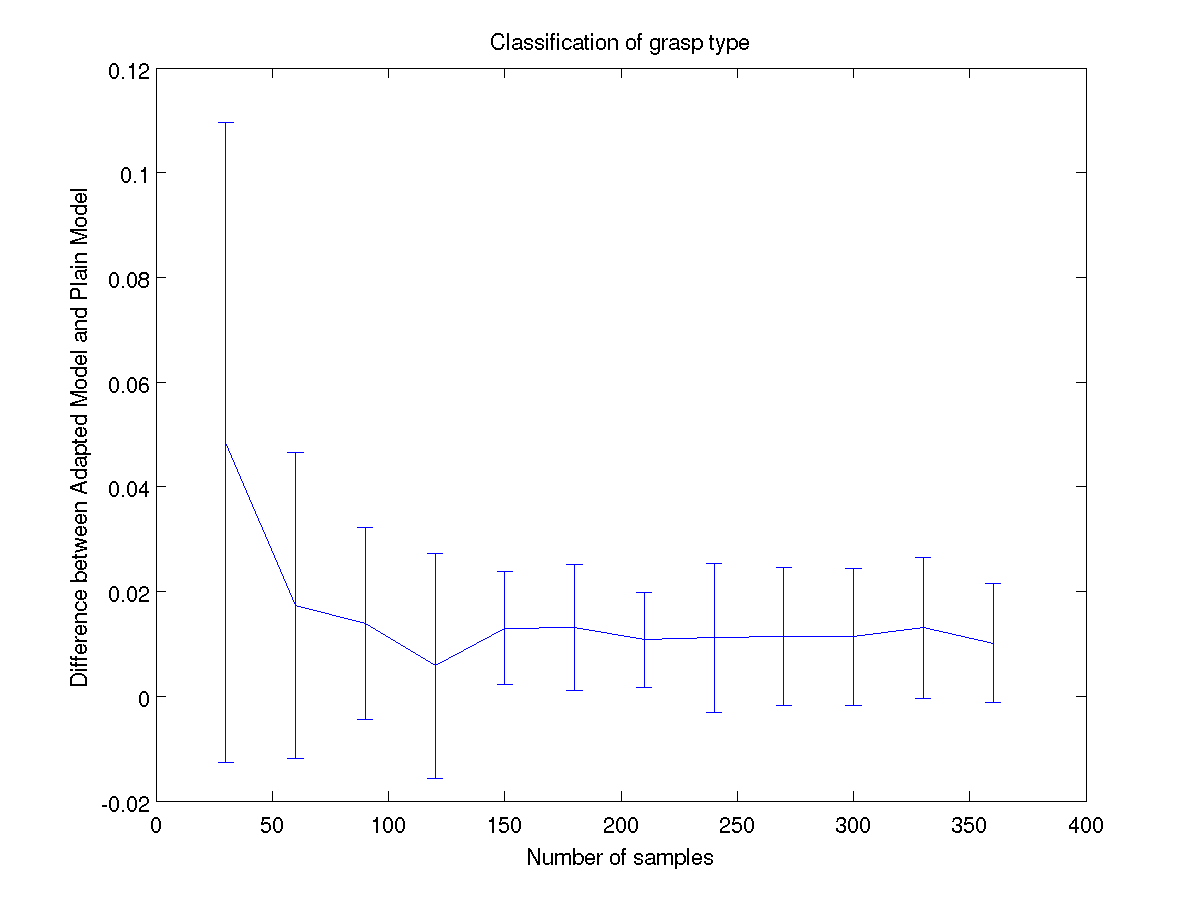
\includegraphics[width=0.95\linewidth]{figs/exp1}
  \caption{Classification results: Difference in performance between \emph{NoAdapt} and our method  on the
 classification of the grasp types.}
  \label{fig:diff_cla}
\end{figure}

\begin{figure*}[ht] \centering
  \begin{tabular}{cc}
    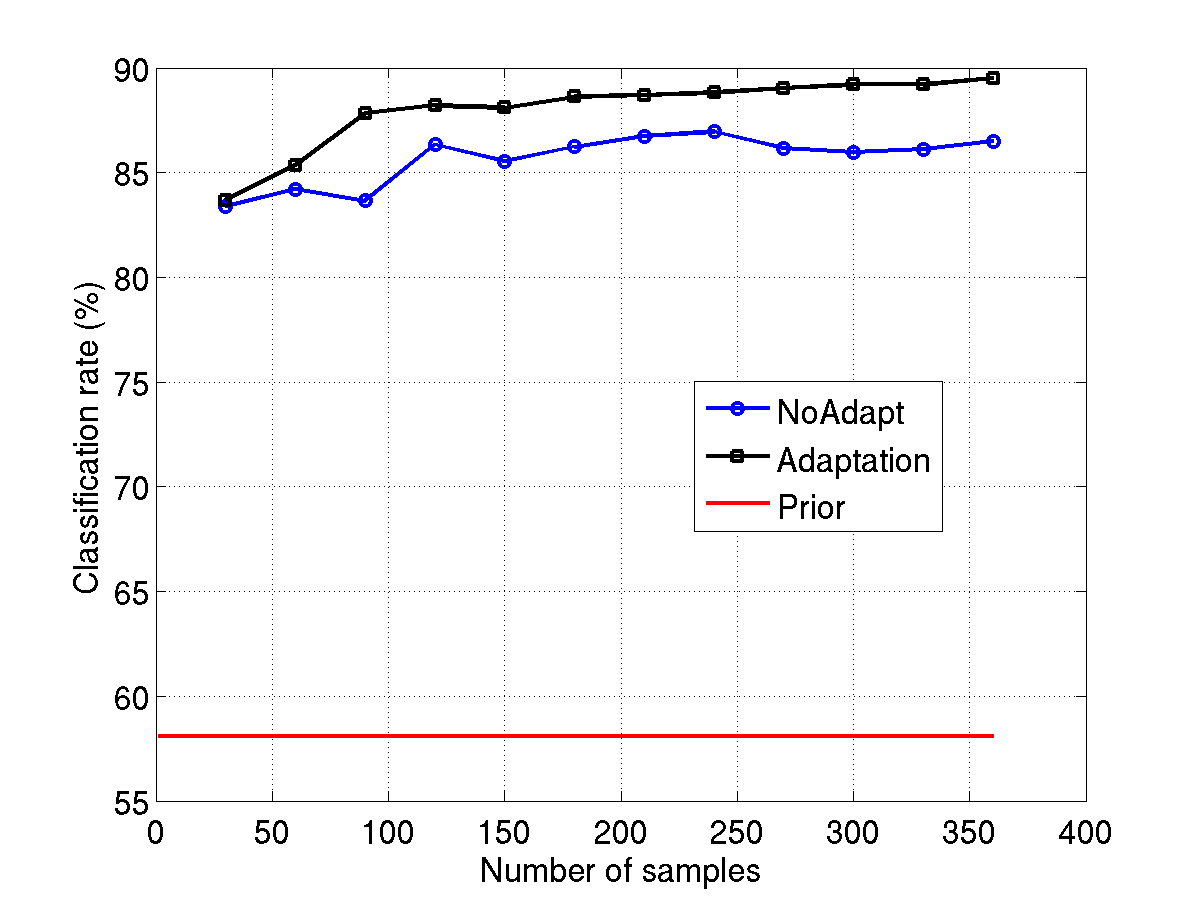
\includegraphics[width=0.45\textwidth]{figs/exp1_abs_best} &
    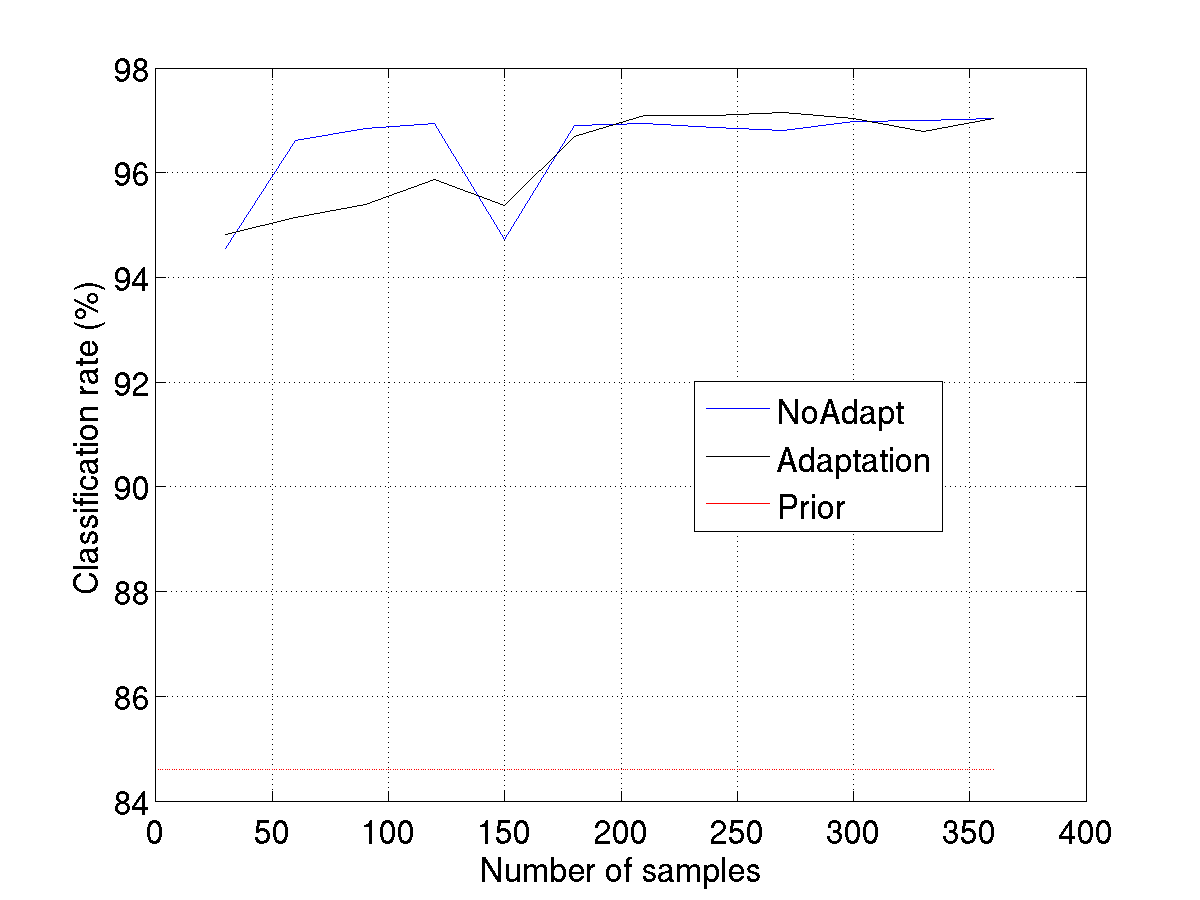
\includegraphics[width=0.45\textwidth]{figs/exp1_abs_worst} \\
    $(a)$ & $(b)$ \\
  \end{tabular}
  \caption{Classification results: $(a)$ Best classification rate gain of the adapted model compared to
 \emph{NoAdapt} and \emph{Prior} on a particular subject; $(b)$ worst performance on another subject.}
  \label{fig:cla_abs}
\end{figure*}

\begin{figure}[ht]
  \centering
  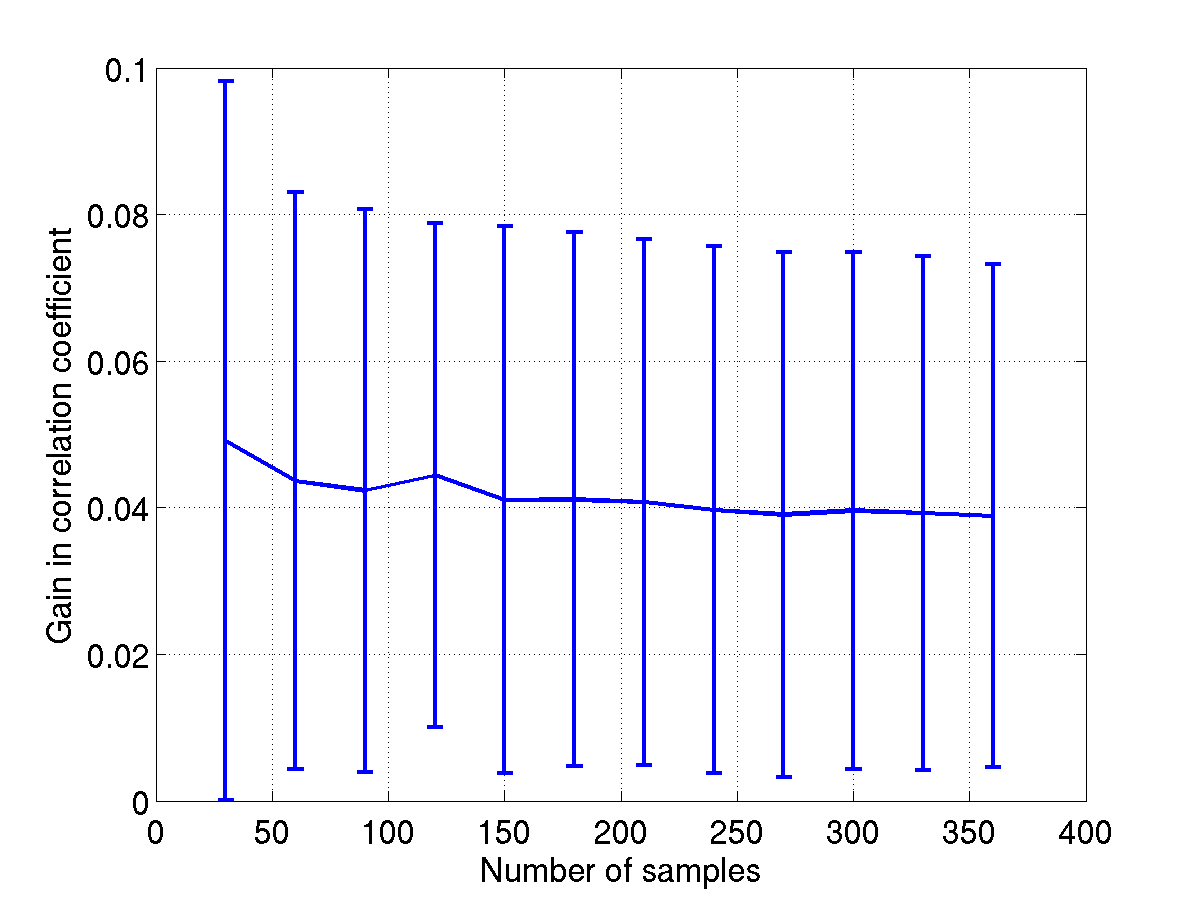
\includegraphics[width=0.95\linewidth]{figs/exp2}
  \caption{Regression experiments: Difference in performance between \emph{NoAdapt} and our method  on the
 regression of the force.}
  \label{fig:diff_reg}
\end{figure}

\begin{figure*}[ht] \centering
  \begin{tabular}{cc}
    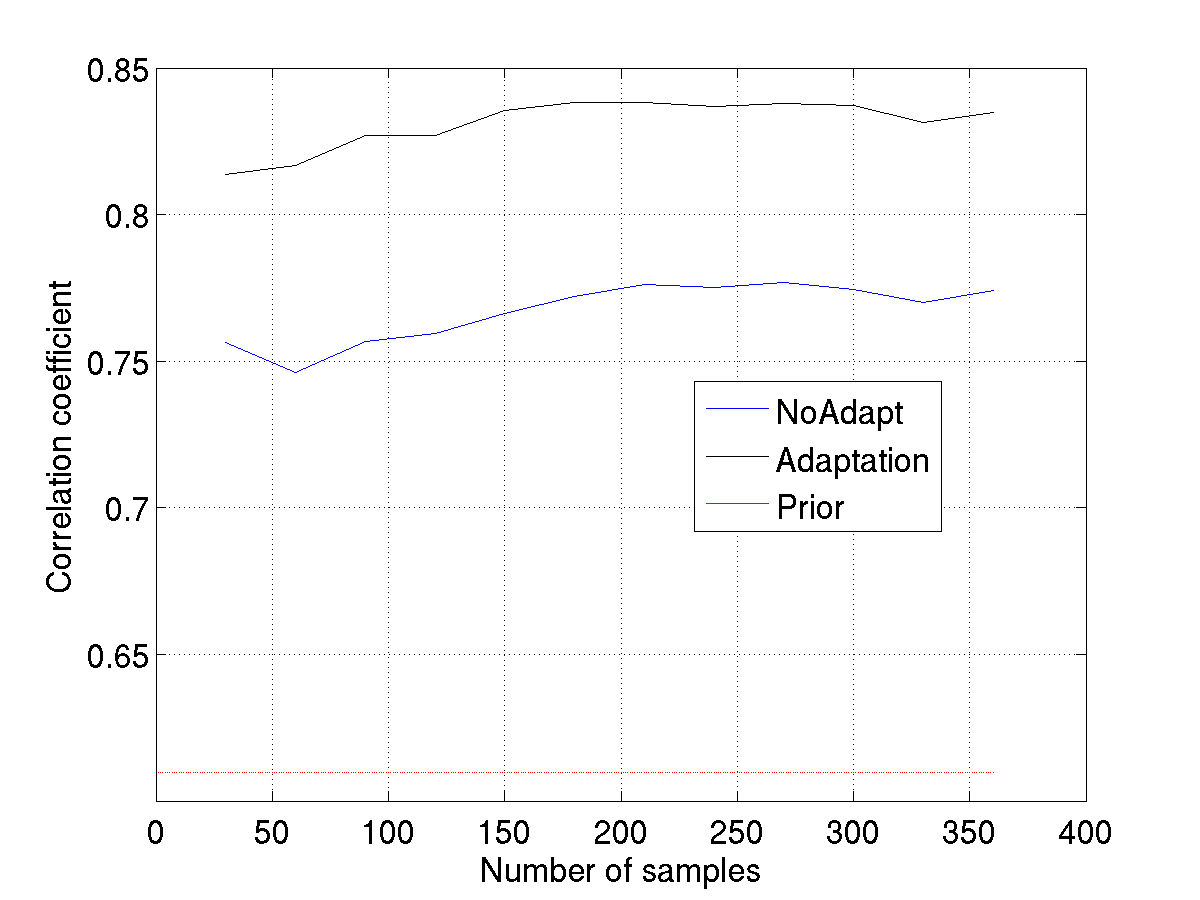
\includegraphics[width=0.45\textwidth]{figs/exp2_abs_best} &
    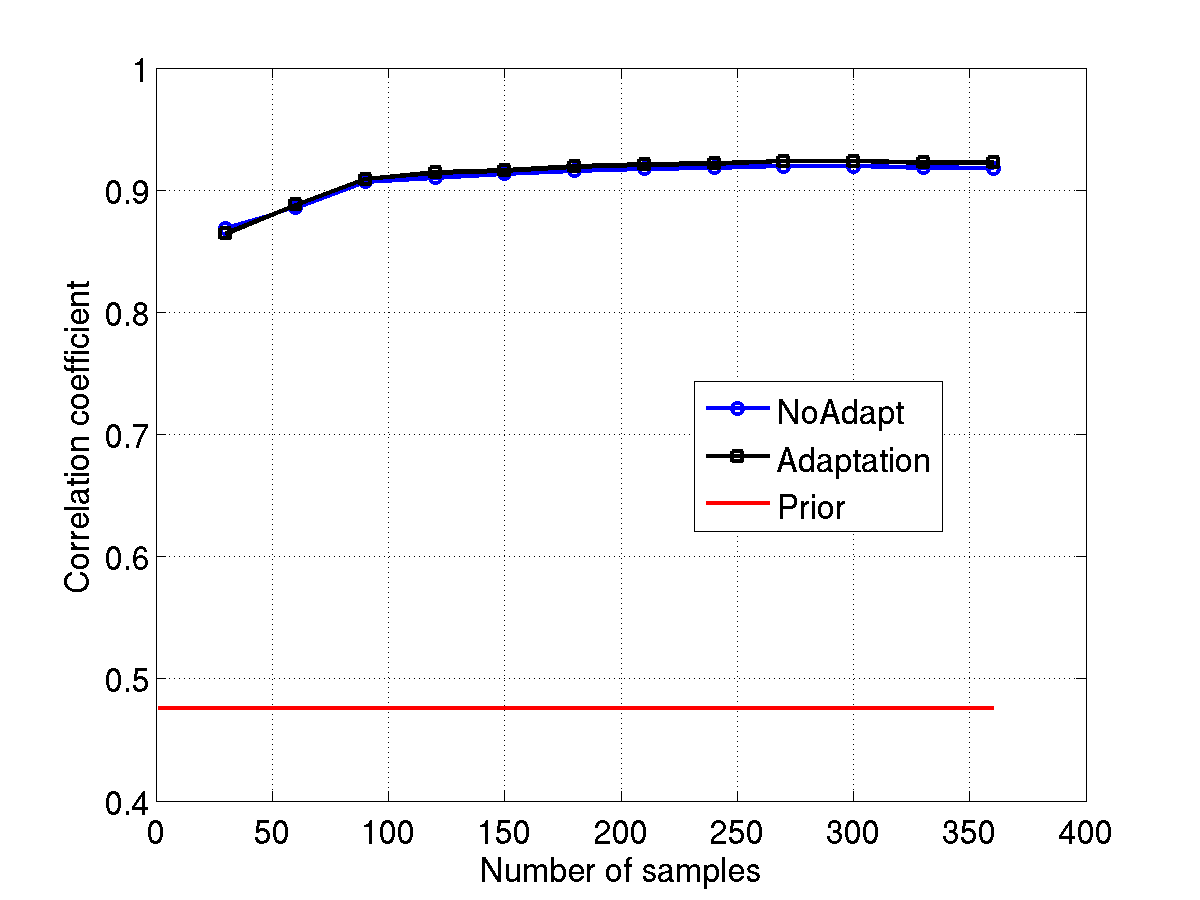
\includegraphics[width=0.45\textwidth]{figs/exp2_abs_worst} \\
    $(a)$ & $(b)$ \\
  \end{tabular}
  \caption{Regression experiments: $(a)$ Best correlation coefficient gain of the adapted model compared to \emph{NoAdapt}
 and \emph{Prior} on a particular subject; $(b)$ worst performance on another subject.}
  \label{fig:reg_abs}
\end{figure*}
